\documentclass[24pt,pdf,hyperref={unicode},aspectratio=169]{beamer}
\usepackage[utf8]{inputenc}
\usepackage{aiml}

\begin{document}

\section{Подбор кодирования в двух классических задачах}


\begin{frame}\frametitle{Задача коммивояжера}

\uncover<+->{
{\bf Дано}: граф $G=(V,E)$ и функция $W:E\rightarrow\mathbb{R}$.\\[0.3cm]

{\bf Найти}: проходящий единожды по всем вершинам цикл $C=(e_1,\ldots,e_n)$ такой, что $\sum_{e\in C} W(e)\rightarrow \min$\\[0.3cm]
}

\uncover<+->{ {\bf Кодирование:} }\uncover<+->{$S: V\rightarrow V$, биекция (перестановка)}\\[0.3cm]

\uncover<+->{{\bf Мутация}:}\uncover<+->{перестановка соседних элементов}\\[0.3cm]

\uncover<+->{{\bf Скрещивание}:}

\uncover<+->{$$
c(S_1,S_2)=S_1\circ S_2
$$}

\uncover<+->{{\bf Оценка}: }\uncover<+->{$$
f(C)=\left(\sum_{e\in C} W(e)\right)^{-1}
$$}

\end{frame}

\begin{frame}\frametitle{Система уравнений}

\uncover<+->{
{\bf Дано}: система уравнений вида $\left\{ f_i(x_1,\ldots,x_n)=0\right.$, например:

$$
\left\{\begin{array}{c c c}
        x_1^2 + \sin x_2 & = &0 \\
        e^{x_1+x_2}-x_1x_2 & = & 0 \\
       \end{array}\right.
$$\\[0.3cm]

{\bf Найти}: решение системы уравнений\\[0.3cm]
}

\uncover<+->{{\bf Кодирование}: }\uncover<+->{$(x_1,\ldots,x_n)$}\\[0.3cm]

\uncover<+->{{\bf Мутация}: }\uncover<+->{$(c_1x_1,\ldots,c_nx_n)$, $c_i\in[1-\varepsilon,1+\varepsilon]$}\\[0.3cm]

\uncover<+->{{\bf Скрещивание}: }\uncover<+->{обычное}\uncover<+->{, или $
\frac{(x_1,\ldots,x_n)+(y_1,\ldots,y_n)}{2}$}\\[0.3cm]

\uncover<+->{{\bf Оценка}: }\uncover<+->{$$
\left(1+\sum_{i=0}^{n}\left|f_i(x_1,\ldots,x_n)\right|\right)^{-1}
$$}

\end{frame}

\section{Сегментация изображений и многокритериальная оптимизация}

\begin{frame}\frametitle{Сегментация изображений}

\uncover<+->{
{\bf Дано}: экспериментальная база, состоящая из пикселей, отнесенных к определенным классам\\[0.3cm]

{\bf Найти}: способ правильно относить пиксели извне базы данных к классам  \\[0.3cm]
}


\uncover<+->{ {\bf Кодирование}: }\uncover<+->{ $(h_i,s_i,b_i)$ для каждого класса }  \\[0.3cm]

\uncover<+->{ {\bf Мутация и скрещивание} как для SET PARTITION} \\[0.3cm]

\uncover<+->{ {\bf Оценка}}\uncover<+->{ многокритериальная:

$p_i$ -- процент пикселей, попавших в свой класс

$n$ -- количество прямоугольников

$f=p_i+1/n$
}

\end{frame}


\begin{frame}

\begin{tikzpicture}[x=2cm,y=-1cm]

\uncover<+->{
\node (a) at (-0.5,0) {$sat\in[0,1]$};
}
\uncover<+->{
\node (b) at (1,0) {$2^{\lfloor 32\cdot sat\rfloor}$};
\draw[->] (a) -- (b);
}
\uncover<+->{
\node (c) at (3,0) {$\begin{array}{|c|c|c|c|c||c|c|}\hline 0&0&1&0&0&0&0 \\ \hline \end{array}$};
\draw[->] (b) -- (c);
}
\uncover<+->{
\node at (3,1) {$\begin{array}{|c|c|c|c|c||c|c|}\hline 0&1&1&1&0&0&0 \\ \hline \end{array}$};
}
\uncover<+->{
\node at (1.7,0.5) {$AND$};
\draw (2,1.6) -- (4,1.6);
}
\uncover<+->{
\node at (3,2) {0 или не 0};
}
\end{tikzpicture}

\end{frame}


\section{Об одной прикладной задаче}

\begin{frame}\frametitle{Функциональное уравнение}

\uncover<+->{
{\bf Дано}: функция, определяемая дифференциальным уравнением $f(t)=\Phi[C(T),U(T),\rho(T)](t)$ и экспериментально измеренные значения этой функции $g(t)$.\\[0.3cm]

{\bf Найти}: функции $C(T)$, $U(T)$ и $\rho(T)$, обеспечивающие согласование эксперимента и теории \\[0.3cm]
}


\uncover<+->{ {\bf Кодирование}: }\uncover<+->{$C(T)=(a_C,b_C,c_C)$, $U(T)=(a_U,b_U,c_U)$ $\rho(T)=(a_\rho,b_\rho,c_\rho)$}  \\[0.3cm]

\uncover<+->{ {\bf Мутация и скрещивание} как для системы уравнений} \\[0.3cm]

\uncover<+->{ {\bf Оценка}:}\uncover<+->{
$$
\left(1+\int_t|f(t)- g(t)|dt \right)^{-1}
$$}
\end{frame}

\begin{frame}
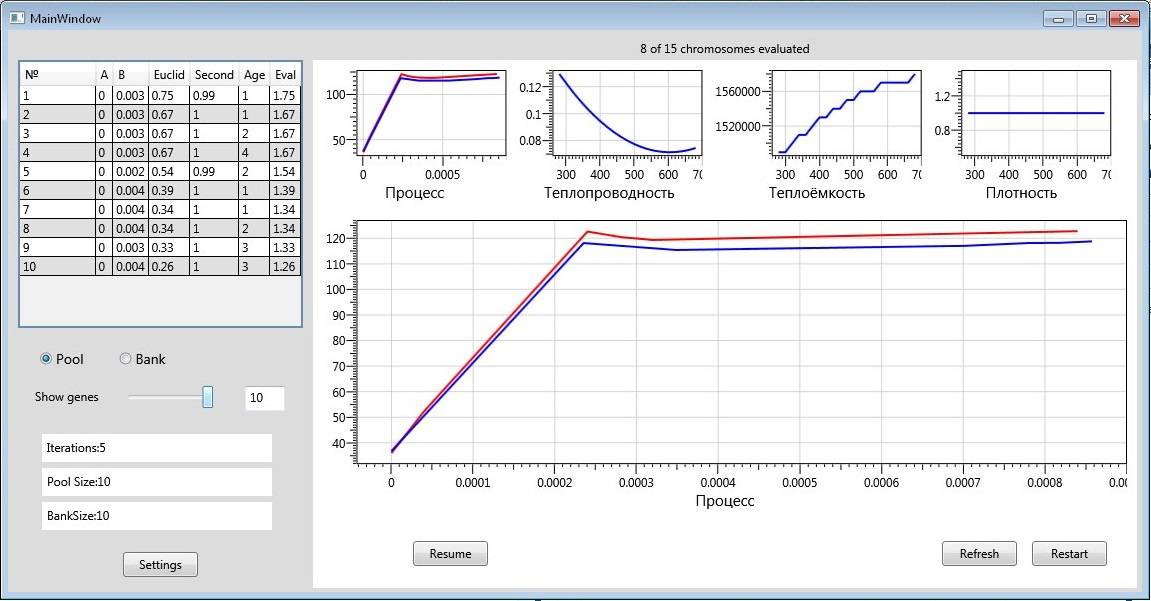
\includegraphics[width=\textwidth]{Images/ga.jpg}
\end{frame}

\end{document}